% Drawing 148/01-5 -- folder 148, batch 01, archive page 17 (PDF page 18).
% Transcription: sous ces deux lignes, deux croquis : un tétraèdre au crayon aux sommets tronqués par de petits cercles ; à droite, un tétraèdre à l'encre dont la subdivision barycentrique est tracée en rouge, avec, en marge :
% Kind: two tetrahedra: truncated vertices; barycentric subdivision. Method 2 (schematic redraw from the facsimile). Status: ok.
% Notes: Left (first pass, checked again on the colour render): a pencil tetrahedron, its vertices ringed by small circles (truncation), the hidden edge in short dashes, a stroke across the upper part; the pencil shading is left out. Right, re-read on a colour crop of p. 17: the ink tetrahedron (four vertices, the five visible edges, small arcs ringing three vertices) and, in red, on each of its two visible faces the triangle joining the midpoints of the sides (midpoints as red points, the strokes from the midpoint of the common edge heavy) with a black dot in the middle of each of its sides, each dot joined in red to the opposite vertex of the face.
% Coordinates: 1 unit = 1 mm = 1/100 of the crop width (bbox in page fractions: [0.19, 0.11, 0.74, 0.28]).
% Redrawn by Claude (claude-opus-5-5), issue #73, 2026-11-07; not checked by a human; not compiled (no TeX in the session).
% Rights: reproduces part of the work -- behind RENDER_TRANSCRIPTS, never published by itself.
\documentclass[tikz,border=3pt]{standalone}
\usepackage{amsmath,amssymb}
\usetikzlibrary{patterns,arrows.meta}
\tikzset{Rd/.style={red!85!black}, pencil/.style={black!45}, struck/.style={black!35}, mark/.style={circle,draw,inner sep=1.3pt}, pt/.style={circle,fill,inner sep=0.9pt}, opt/.style={circle,draw,fill=white,inner sep=1.1pt}}
\begin{document}
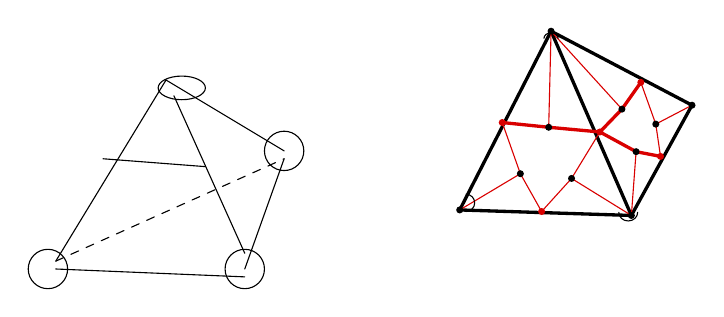
\begin{tikzpicture}[x=1mm,y=1mm,line cap=round,line join=round,font=\scriptsize]
\draw (28,-10) -- (14,-33);
\draw (14,-34) -- (38,-35);
\draw (38,-34) -- (43,-20);
\draw (28,-10) -- (43,-19);
\draw (29,-12) -- (38,-32);
\draw[dashed] (14,-33) -- (43,-20);
\draw (20,-20) -- (33,-21);
\draw (30,-11) ellipse[x radius=3, y radius=1.5];
\draw (13,-34) circle[radius=2.5];
\draw (38,-34) circle[radius=2.5];
\draw (43,-19) circle[radius=2.5];
\draw[very thick] (76.9,-3.8) -- (65.3,-26.5);
\draw[very thick] (65.3,-26.5) -- (87.1,-27.2);
\draw[very thick] (87.1,-27.2) -- (94.8,-13.2);
\draw[very thick] (76.9,-3.8) -- (94.8,-13.2);
\draw[very thick] (76.9,-3.8) -- (87.1,-27.2);
\draw[Rd,very thick] (70.7,-15.4) -- (76.6,-16) -- (83.1,-16.6);
\draw[Rd,very thick] (83.1,-16.6) -- (85.9,-13.7) -- (88.3,-10.3);
\draw[Rd,very thick] (83.1,-16.6) -- (87.7,-19.1) -- (90.8,-19.7);
\draw[Rd] (70.7,-15.4) -- (73,-21.9) -- (75.7,-26.7);
\draw[Rd] (83.1,-16.6) -- (79.5,-22.5) -- (75.7,-26.7);
\draw[Rd] (88.3,-10.3) -- (90.2,-15.6) -- (90.8,-19.7);
\draw[Rd] (76.9,-3.8) -- (76.6,-16);
\draw[Rd] (76.9,-3.8) -- (85.9,-13.7);
\draw[Rd] (65.3,-26.5) -- (73,-21.9);
\draw[Rd] (87.1,-27.2) -- (79.5,-22.5);
\draw[Rd] (87.1,-27.2) -- (87.7,-19.1);
\draw[Rd] (94.8,-13.2) -- (90.2,-15.6);
\node[pt,Rd] at (70.7,-15.4) {};
\node[pt,Rd] at (83.1,-16.6) {};
\node[pt,Rd] at (88.3,-10.3) {};
\node[pt,Rd] at (75.7,-26.7) {};
\node[pt,Rd] at (90.8,-19.7) {};
\node[pt] at (76.6,-16) {};
\node[pt] at (73,-21.9) {};
\node[pt] at (79.5,-22.5) {};
\node[pt] at (85.9,-13.7) {};
\node[pt] at (90.2,-15.6) {};
\node[pt] at (87.7,-19.1) {};
\node[pt] at (76.9,-3.8) {};
\node[pt] at (65.3,-26.5) {};
\node[pt] at (87.1,-27.2) {};
\node[pt] at (94.8,-13.2) {};
\draw (77.8,-4.7) arc[start angle=0, end angle=180, x radius=0.9, y radius=0.7];
\draw (66.1,-26.7) arc[start angle=-90, end angle=90, x radius=1.1, y radius=1.1];
\draw (85.5,-26.8) arc[start angle=180, end angle=360, x radius=1.2, y radius=1.1];
\end{tikzpicture}
\end{document}
